\chapter{Lab 3: Bouncing Ball \\
\index{Lab 3}
\index{introduction}
\label{Introduction}}

\section{Lessons Learned \label{Section::Lessons Learned}}
    We learned how to use an FPGA to write to a display and how it changes with each cycle of the clock and then combined it with a previous lab (Adder Lab) to change the speed of the ball by flipping switches on the board and then we changed the color of the ball. After that, the final alteration that we made was to convert the moving ball to a pong style game with a paddle controlled by a dial to prevent the ball from touching the bottom of the screen. 

    We used the VGA port on the board to connect to a television. What this lab was teaching us was how to use different types of add ons to the board and how we would need to alter the code within. 
 \section{Schematics and Block Diagrams}
    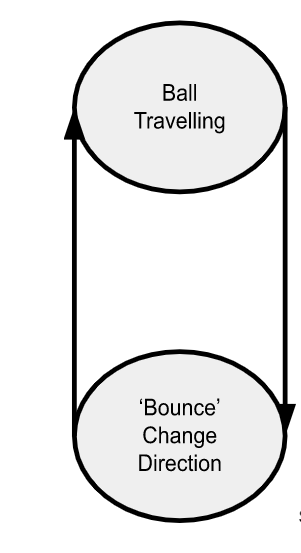
\includegraphics[width=100mm]{lab3/Lab3t.png}
    \emph{Figure 3.1: Input and Output of the System}
    
 \section{VHDL Architecture}
    \begin{verbatim}
    ## Clock signal
    set_property -dict { PACKAGE_PIN E3    IOSTANDARD LVCMOS33 } [get_ports { clk_in }]; #IO_L12P_T1_MRCC_35 Sch=clk100mhz
    create_clock -add -name sys_clk_pin -period 10.00 -waveform {0 5} [get_ports {clk_in }];
            
    ##VGA Connector            
    set_property -dict { PACKAGE_PIN A3    IOSTANDARD LVCMOS33 } [get_ports { vga_red[0] }]; #IO_L8N_T1_AD14N_35 Sch=vga_r[0]
    set_property -dict { PACKAGE_PIN B4    IOSTANDARD LVCMOS33 } [get_ports { vga_red[1] }]; #IO_L7N_T1_AD6N_35 Sch=vga_r[1]
    set_property -dict { PACKAGE_PIN C5    IOSTANDARD LVCMOS33 } [get_ports { vga_red[2] }]; #IO_L1N_T0_AD4N_35 Sch=vga_r[2]
            
    set_property -dict { PACKAGE_PIN C6    IOSTANDARD LVCMOS33 } [get_ports { vga_green[0] }]; #IO_L1P_T0_AD4P_35 Sch=vga_g[0]
    set_property -dict { PACKAGE_PIN A5    IOSTANDARD LVCMOS33 } [get_ports { vga_green[1] }]; #IO_L3N_T0_DQS_AD5N_35 Sch=vga_g[1]
    set_property -dict { PACKAGE_PIN B6    IOSTANDARD LVCMOS33 } [get_ports { vga_green[2] }]; #IO_L2N_T0_AD12N_35 Sch=vga_g[2]
    
    set_property -dict { PACKAGE_PIN B7    IOSTANDARD LVCMOS33 } [get_ports { vga_blue[0] }]; #IO_L2P_T0_AD12P_35 Sch=vga_b[0]
    set_property -dict { PACKAGE_PIN C7    IOSTANDARD LVCMOS33 } [get_ports { vga_blue[1] }]; #IO_L4N_T0_35 Sch=vga_b[1]
            
    set_property -dict { PACKAGE_PIN B11   IOSTANDARD LVCMOS33 } [get_ports { vga_hsync }]; #IO_L4P_T0_15 Sch=vga_hs
    set_property -dict { PACKAGE_PIN B12   IOSTANDARD LVCMOS33 } [get_ports { vga_vsync }]; #IO_L3N_T0_DQS_AD1N_15 Sch=vga_vs
    \end{verbatim}
 \section{VHDL Models}
 
    \begin{enumerate}
        \item Data Flow Architecture
            \begin{verbatim}
                ball.vhd
                    input: pixel row and column
                    output: color of that pixel (RGB)
                vga_sync.vhd
                    input: pixel clock, color in (RGB, background),
                    output: Pixel Location, color out (RGB)
                vga_top.vhd
                    input: clock
                    output: color of background (RGB)
            \end{verbatim}
        \item Structural Modeling
            \begin{verbatim}
                vga_top 
                    add_ball : ball
                    vga_driver : vga_sync
                    clk_wiz_0)inst : clk_wiz_0
                        U0 : clk_wiz_clk_wiz
            \end{verbatim}
        \item Behavioral Models
            The program has one input and that is switches on the board which dictate the speed of the ball on the screen. This is primarily a binary conversion from the number of switches up to 7 turned on. 
     \end{enumerate}

 \section{VHDL Component Reuse}
    The program reuses the FPGA board, switches on the board and it also reuses some of the logic from earlier labs. However, most of the lab was new and it is due to the fact that it is writing to the VGA port. We had to change the size and color of the ball so that was changed between iterations and the ball was able to move vertically as well as horizontally. 
 \section{VHDL Digital Circuits}
    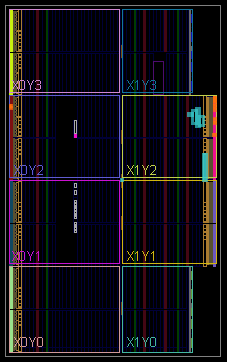
\includegraphics[width=100mm]{lab3/lab3imgthing.png}
    \emph{Figure 3.2: Digital architecture and setup of the circuit}
 \section{State Machines}
    The circuit is idle while booting, however the program runs until turned off due to the nature of the program (bouncing ball). 
 \section{Testing}
    We tested it by inputting different values for the speed and color of the ball and then reprogramming the board to see how it will affect the display. 
